\documentclass[11pt,a4paper]{article}
\usepackage[margin=2.2cm]{geometry}
\usepackage{graphicx,booktabs,amsmath,siunitx,hyperref,caption,float}
\graphicspath{{figures/}{../reports/retests/20261025T172218Z/}}
\captionsetup{justification=raggedright,singlelinecheck=false}
\sisetup{group-separator={,},group-minimum-digits=4}
\hypersetup{colorlinks=true,linkcolor=black,urlcolor=blue,citecolor=black}

\title{Data-driven surrogate for the stress response of AlSi10Mg\\
\large Multiscale modelling of an additively manufactured wing-rib bracket — ML component}
\author{Team 8}
\date{October 2026}

\begin{document}
\maketitle

\begin{abstract}
We trained a small neural-network surrogate that predicts the von Mises stress response $S_{vm}$ of AlSi10Mg along the operational strain $E_{11}$, given temperature, strain rate, density and shear modulus. The final predictor averages five 5--16--16--1 tanh networks (385 parameters each). On a fixed split of 37 held-out simulations, the mean per-curve RMSE is 0.0591 (worst 0.1133, case 45). Performance is much weaker when whole temperature/rate conditions are held out (mean 6.79), so the model closely reproduces the 37 related test curves, but its reliability at other input combinations, even inside the numerical ranges, is not established. Units are inferred, the held-out set is not fully blind, and the link from material porosity to the aerodynamic coefficient of lift $C_L$ has not been established. These limits are stated throughout.
\end{abstract}

\section{Introduction and scope}
The wider project studies how porosity in an additively manufactured AlSi10Mg wing-rib bracket affects structural and aerodynamic behaviour. This report covers only the machine-learning component: a fast surrogate for the material's simulated stress response, intended to replace repeated material simulations inside a larger multiscale workflow. The structural (ANSYS) analysis is a teammate's work and is not reported here. Throughout, $C_L$ means the coefficient of lift; no lift labels exist in the material data, so this report makes no aerodynamic prediction.

\section{Data}
The professor's design matrix planned 108 simulations; 73 were available, containing \num{2197000} raw history rows. Temperature coverage is uneven: 27 cases at 30, 27 at 100, 19 at 200 and none at 300 (units inferred as \si{\celsius}). Each case also varies strain rate ($10^{-5}$ to $10^{-3}$, inferred \si{\per\second}), density (2488.05 to 2700) and shear modulus $G$ (23313.95 to 25300).

The target is $S_{vm}$ along operational $E_{11}$, not $S_{CAU11}$. Each history was interpolated onto a common grid of 120 $E_{11}$ values from 0.0002 to 0.0999, so long, slow-rate runs do not dominate by row count. The histories do not show a conventional zero-stress elastic loading segment, so the surrogate should not be read as a constitutive law.

\section{Method}
\subsection{Split and leakage control}
We used one fixed random split by simulation (seed 42): 36 training cases and 37 test cases, following the professor's requested 50/50 split as closely as 73 cases allow. All points from one simulation stay in one partition, and scalers were fitted on training cases only. The 36 training cases give \num{4320} query points; these are not independent simulations. Earlier exploration used all the data, so the 37 test cases were excluded from final fitting but are \emph{not} a fully blind holdout.

\subsection{Model}
Each network takes five inputs (temperature, $\log_{10}$ strain rate, density, $G$, and the query $E_{11}$) and outputs one $S_{vm}$ value. The architecture is 5--16--16--1 with tanh hidden layers and a linear output (385 parameters per network, \num{1925} in total). Five networks with seeds 0--4 are trained with scikit-learn~\cite{sklearn} using L-BFGS~\cite{lbfgs} and L2 penalty $\alpha = 0.001$, and their predictions are averaged. This is a data-driven surrogate: there is no physics-informed loss term.

\subsection{Model selection}
Candidates were compared on training-side evidence only: case-wise cross-validation and a condition holdout (whole temperature/rate groups removed). Table~\ref{tab:candidates} lists the saved results. The query MLP was chosen because it had the best condition-holdout error, which matters most for use beyond the sampled conditions, while its case-CV error was competitive. A PCA + Gaussian-process~\cite{gp} model was better on case CV but much worse when conditions were held out.

\begin{table}[H]\centering
\caption{Saved training-side comparison. Case CV is the mean curve RMSE over the 36 training cases; condition holdout is the unweighted mean of nine group-mean curve RMSEs (one per temperature/rate group), so it is neither a pooled nor a case-weighted error. Both are saved results, not a fresh evaluation of the delivered model.}
\label{tab:candidates}
\begin{tabular}{lrr}\toprule
Candidate & Case CV & Condition holdout\\\midrule
Query MLP (selected) & 1.158 & 6.794\\
PCA + GP (6 components) & 0.664 & 10.962\\
MLP/GP blend & 0.867 & 7.983\\
Physics-style-input MLP & 1.536 & 8.609\\
PCA-coefficient MLP (4) & 2.269 & 11.086\\
PCA-coefficient MLP (6) & 2.004 & 11.205\\\bottomrule
\end{tabular}
\end{table}

\section{Results}
On the 37 test cases the delivered model gives the errors in Table~\ref{tab:test}. Figure~\ref{fig:test} shows two of them, including the worst.

\begin{table}[H]\centering
\caption{Test-set errors of the final model (inferred stress units).}
\label{tab:test}
\begin{tabular}{lr}\toprule
Metric & Value\\\midrule
Mean per-curve RMSE & 0.05909\\
Median per-curve RMSE & 0.05057\\
Worst curve RMSE (case 45) & 0.11331\\
Mean per-curve MAE & 0.04900\\
Pooled RMSE (all points) & 0.06486\\
Largest single-point error & 0.28832\\\bottomrule
\end{tabular}
\end{table}

\begin{figure}[H]\centering
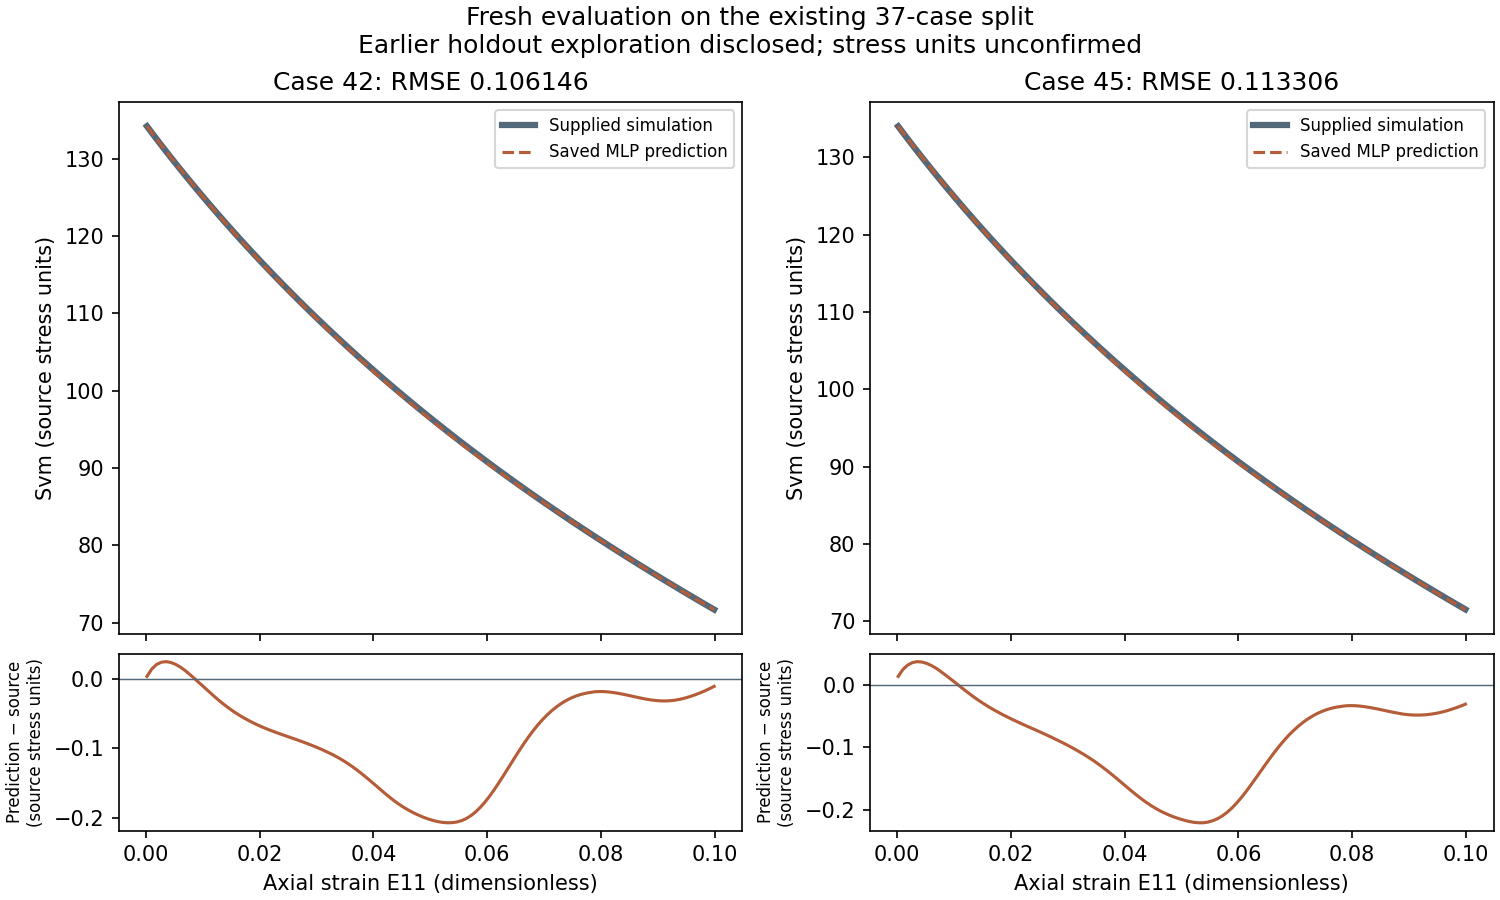
\includegraphics[width=0.92\linewidth]{test_curves.png}
\caption{Predicted vs.\ simulated $S_{vm}$ for test cases 42 and 45, with residuals below (fresh retest, 25 Oct 2026). Case 45 is the worst of the 37 test curves.}
\label{fig:test}
\end{figure}

\paragraph{Generalisation to new conditions.} Holding out whole temperature/rate groups raises the error to 6.79 (unweighted mean over the nine groups), about a hundred times the random-split error (Figure~\ref{fig:loco}). The hardest group, 200 at $10^{-5}$, gives 23.53. Its only available case (60) lies in the training half. The low random-split error therefore mainly shows interpolation between closely related simulated conditions.

\begin{figure}[H]\centering
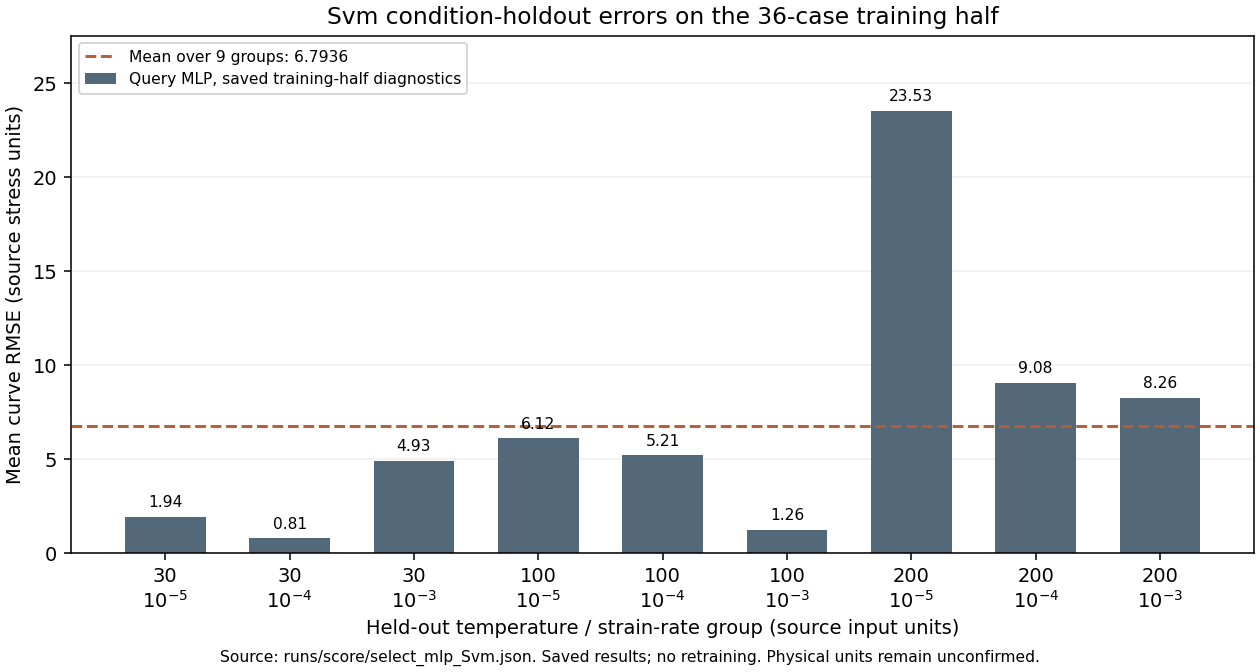
\includegraphics[width=0.75\linewidth]{condition_holdout_Svm.png}
\caption{Saved condition-holdout error of the selected query MLP by temperature/rate group (training half, $\alpha=0.001$), plotted from \texttt{runs/score/select\_mlp\_Svm.json} by \texttt{reports/plot\_report\_diagnostics.py}. This is a plot of saved diagnostics, not a fresh evaluation of the delivered model.}
\label{fig:loco}
\end{figure}

\paragraph{Worked example.} At temperature 100, rate $10^{-4}$, density 2619 and $G = 24541$, the model predicts 136.20912 at the start of the grid, 99.41858716 at $E_{11} = 0.05$ (interpolated) and 75.23194 at the end of the grid.

\paragraph{Reproducibility.} A separate refit with the frozen settings reproduced every weight and prediction exactly in 17.26\,s with no warnings. Thirteen model/parser/runtime unit tests and three live Model Studio tests pass. This is numerical reproducibility in the same environment, not physical, experimental or cross-platform validation.

\section{Discussion}
The surrogate is small, fast and reproducible, and closely reproduces the related test curves. Its reliability at other combinations of inputs is not established, even within the numerical ranges, because some groups are sparse and case 60 is irregular. Its main weakness is extrapolation: with 73 cases spread over three temperatures and three rates, some condition groups have very few cases, and errors grow sharply when a whole group is unseen. We propose adding simulations at the sparse and missing conditions (especially 200 and 300) as the first priority. We have not tested this against changing the model size.

The model predicts stress along operational strain only. Turning it into an input for structural analysis needs the solver's stress/strain definitions, confirmed units and the receiving material model. Any ANSYS-format export remains an unvalidated template until those are confirmed. In particular, it must not invent a zero-origin elastic segment or label a total-strain curve as plastic strain.

\section{Limitations and open questions}
\begin{itemize}
\item Units (\si{\mega\pascal}, \si{\celsius}, \si{\per\second}) are inferred, not confirmed; the solver, material law and stress/strain definitions are unconfirmed.
\item The 37 test cases were seen during earlier exploration, so the test score is not a fully independent generalisation estimate and may be optimistic.
\item Whether density and modulus levels encode porosity, and the mapping if so, is unverified.
\item There are no $C_L$ labels or agreed lift calculation, and the material $\to$ structure $\to$ aerodynamics coupling is undefined.
\item The teammate's ANSYS files, boundary conditions and results have not been inspected; no transfer of predictions into ANSYS has been validated.
\item Stronger generalisation claims need independent experimental data or new simulations.
\end{itemize}

\section{Conclusion}
A five-network MLP ensemble reproduces the simulated AlSi10Mg stress response with a mean test RMSE of 0.059 on related conditions and is exactly reproducible. Predictions at other input combinations, even within the simulated temperature, rate, density and modulus ranges, should be treated as unverified. Extending it to new conditions, porosity effects or lift prediction requires the missing definitions and data listed above.

\section*{Data source}
The simulation data were supplied by the course instructor (unpublished, Team 8 course project, 2026). They are not a public dataset; see \texttt{data/manifest.json} for the case list.

\begin{thebibliography}{9}
\bibitem{sklearn} F.~Pedregosa et al., ``Scikit-learn: Machine learning in Python,'' \emph{J.\ Mach.\ Learn.\ Res.}, 12, 2825--2830, 2011. (Multilayer perceptron, Gaussian process and PCA implementations used.)
\bibitem{lbfgs} D.~C.~Liu and J.~Nocedal, ``On the limited memory BFGS method for large scale optimization,'' \emph{Math.\ Program.}, 45, 503--528, 1989.
\bibitem{gp} C.~E.~Rasmussen and C.~K.~I.~Williams, \emph{Gaussian Processes for Machine Learning}, MIT Press, 2006.
\bibitem{numpy} C.~R.~Harris et al., ``Array programming with NumPy,'' \emph{Nature}, 585, 357--362, 2020.
\bibitem{mpl} J.~D.~Hunter, ``Matplotlib: A 2D graphics environment,'' \emph{Comput.\ Sci.\ Eng.}, 9(3), 90--95, 2007.
\end{thebibliography}

\section*{Software and evidence}
Code: \texttt{src/} (data processing and models) and \texttt{app/} (Model Studio).
Evidence files:
\begin{itemize}
\item \texttt{data/split.json} and \texttt{data/manifest.json}
\item \texttt{runs/score/}
\item \texttt{reports/retests/20261025T172218Z/}
\item \texttt{reports/model\_verification\_20261025.json}
\item \texttt{reports/final\_training\_reproduction\_20261025.json}
\end{itemize}
Repository: \url{https://github.com/SaravananRamar06/MMM-ML}.

\end{document}
